\section{Chapter Overview}
This chapter will cover the network implemented in the course of the project, beginning with the individual \ac{ADPLL}'s composition. A number of attributes for each design will be used to analyse and compare their performance. The impact of some minor architectural changes will also be covered, before the implementation of test network will be described. This chapter will also highlight some pitfalls encountered in the process. The \ac{HDL} Verilog was selected for use in this project due to my prior exposure to that language. 5 MHz was chosen as the target centre frequency for these \ac{ADPLL}s, during initial testing it was discovered that the waveform output via the Digilent Nexys4 development board's \ac{GPIO} ports began to degrade around the 10 MHz mark, preventing accurate analysis.

\section{\acs{ADPLL} Architectures}
Three different architectures of \ac{ADPLL} were implemented in this project for the purposes of testing, and re-use in the future within the research team in \acl{UCD}. Between each design a number of blocks remain constant, as only a single instance of that block was implemented, as variation its design would have negligible impact on the final system. These blocks were the error combiner and frequency divider. The loop filter was implemented both using fractional and integer arithmetic, but as the exact same calculation was performed in both cases there was no impact on the output of the module.

The three architectures chosen for implementation represent a progression from entirely an \ac{FPGA} clock driven system to an \ac{ADPLL} with all components asynchronous with respect to that clock. Therefore the first \ac{ADPLL} design features a clocked oscillator and phase detector, specifically the linear frequency design mentioned in Chapter \ref{chap:3} and the clocked phase detector using a state machine and a bi-directional counter. Skipping over Design 2, the final design used was asynchronous in totality, featuring the \acl{RO} and SigNum/\ac{TDL} phase detector. Design 2 sat between these two, using the \ac{RO} as its oscillator, but retained the clocked phase detector seen in Design 1.

The extensibility of the end product of this project was to the forefront during the design process. Whilst, apart from frequency, there were no guidelines as to what the system should resemble and a number of attributes could be chosen arbitrarily, a future user of this platform could have entirely different requirements or specifications. As such each block was implemented in such a way that changing the number of bits used for a certain signal, the target frequency or swapping between different blocks could be done with the sole requirement of changing Verilog \texttt{localparam}\footnote{A \texttt{localparam} is a constant that cannot be modified in a module instance statement \cite{hdlworks}}s in the module \footnote{Module is the Verilog term for a number of logic elements grouped to provide a certain functionality} in which change was made, which would then propagate to any sub-modules affected. Starting the design process with this in mind was a major benefit at later stages when frequent modifications were being made to test their impact, or when changing between \ac{ADPLL} designs.

\subsection{Generic Components}
As mentioned in the chapter overview, a number of components were used in all \ac{ADPLL}s implemented, as changes in their design would not impact the overall system.
\subsubsection{Error Combiner}
The error combiner in this design had a number of requirements in order to be suitable for use in both a single \ac{ADPLL} as well as a network operating in both uni- and bi-directional modes, alongside modifications which would change the widths of the error signals requiring averaging. The module was implemented on the basis that the \ac{LF} input width would be identical to the phase detector output width.

The error combiner was designed to take in up to four error signals, all of an identical width which defaults to eight, and four weights to apply in the summation process. A weighted summation is performed by multiplying each error signal by the weight and adding the results together. Regardless of the number of input error signals, a division by four is then performed in order to compute the average error, done by shifting the value right by two. In a \ac{HDL}, unlike C programming or similar, a shift requires no computation and is instead implemented by performing a part-selection. As all error signals are two's complemented signed integers, the error combination process is also carried out using signed values. The code implementing the error combiner can be found in \textsc{ErrorCombiner.v}, attached in Appendix \ref{adx:code} Listing \ref{lst:error_combiner}.

\subsubsection{Frequency Divider}
The frequency divider is implemented using ``Divider 2'' from Chapter \ref{chap:3}, as only divisions ratios of 2, 4 and 8 were selected for use in the testing process. For ease of testing, the divider had outputs representing each of these division ratios simultaneously, which could be multiplexed between at runtime if so desired. A fourth output passed the input through unmodified, allowing for the divider to be removed without regeneration of the \ac{FPGA} configuration.
\begin{figure}[h]%
	\centering
	
\includegraphics[width=0.6\textwidth]{../divider2}
	\caption[Frequency divider \ac{RTL} diagram]{Frequency divider \ac{RTL} diagram.}
	\label{fig:divs_impl}
\end{figure}

\subsubsection{Loop Filter}
Two \acl{LF}s were implemented, both as \ac{IIR} filters. \ac{FIR} was dismissed due to the extra hardware required to implement the calculations within a single clock cycle, as the \ac{LF} is clocked using the oscillator output, and the greater difficulty of gain adjustment compared to an \ac{IIR}. Clocking on using the generated signal ensures that the discrete time integration is only carried out once per phase comparison. A pitfall that may be encountered implementing an \ac{ADPLL} featuring a divider is not clocking the module on the divided clock, which will result in the integration being carried out at the oscillator output frequency.

Each of integer and fixed-point arithmetic were used to implement a filter respectively, however both designs are interchangeable as they perform the integration identically, given the same proportional and integral gains. All testing was carried out using integer arithmetic, as in Figure \ref{fig:integer_lf}, however the interchangeability will be confirmed later in this chapter, in Section \ref{section:minor_variations}. Additionally the \ac{LF} supports variation of both \acs{ki} and \acs{kp} at runtime, however, if a static value is desired the runtime variation may be disabled using a \texttt{parameter}\footnote{Parameters are constant values that may be changed at compile time, or in the module instance statement \cite{hdlworks2}}.
\begin{figure}[h]%
	\centering
	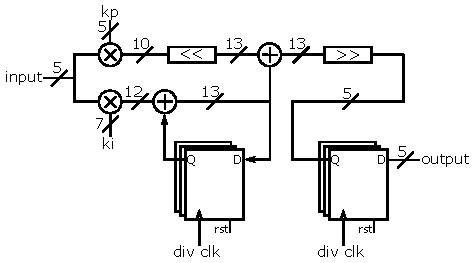
\includegraphics[width=0.8\textwidth]{../integer_lf} 
	\caption[\acl{LF} implemented using integer arithmetic \ac{RTL} diagram]{\acl{LF} implemented using integer arithmetic \ac{RTL} diagram (signal widths using default values).}
	\label{fig:integer_lf}
\end{figure}

Figure \ref{fig:integer_lf} contains an \ac{RTL} diagram describing the implementation. Important to note is the shift applied to the result of the multiplication by \acs{kp} which, as the integration is performed with a larger width to avoid accumulator overflow, preserves the intended relationship between proportional and integral gains. The value of $k_p$ and $k_i$ can be computed using the following formulae:
\begin{gather}
\text{Proportional gain} = k_p\times 2^{-path\_width\_change\_p} \\
path\_width\_change\_p = lsh\_width - rsh\_width \\
lsh\_width = ki\_width - kp\_width  \\
rsh\_width = error\_width + kp\_width + lsh\_width - control\_code\_width \\
\text{Integral gain} = k_i\times 2^{-path\_width\_change\_i} \\
path\_width\_change\_i = - rsh\_width
\end{gather}
In the example system shown in Figure \ref{fig:integer_lf} the proportional gain can be computed as $k_p\times 2^{3-8} = \frac{k_p}{32}$ and the integral gain is $k_i\times 2^{-8} = \frac{k_i}{128}$.
The Verilog implementation of the \ac{LF} using integer arithmetic can be found in \textsc{LoopFilter.v}, attached in Appendix \ref{adx:code} Listing \ref{lst:loop_filter}.

\subsection{\acs{ADPLL} Design 1}
\acs{ADPLL} Design 1 is comprised of the aforementioned generic components and \ac{FPGA} clocked implementations of the \ac{PFD} and \ac{DCO}. This was the first solution addressed in the course of this project as it is the simplest to both implement and test, as all aspects of the \ac{ADPLL} are driven by the \ac{FPGA} clock. Compared to later designs utilising the \ac{RO}, Vivado simulations could be carried out, with accurate timing behaviour, depicting the locking process. The \ac{DCO} was chosen to be linear in frequency in order to obtain a square wave output as it was not yet known whether the varying pulse width of a period linear design would cause a problem in modules which, at that stage in the project, had not yet been designed. Indeed, a later discarded version of the \ac{FPGA} clocked \ac{PFD} relied on equal low and high times. The \ac{PFD} itself was implemented using a Moore type \ac{FSM} driving a up-down counter to convert the time between rising edges to a digital signal.

\subsubsection{\acl{DCO}}
As the \ac{FPGA} clocked, linear frequency oscillator is based on the use of counters, the first stage in its design was the decisions as to their required widths. The equation given previously is used here, with the control code set to zero in order to obtain the centre frequency, and 5 MHz as the target \ac{DCO} frequency:
\begin{align}
f_{osc} &= f_{FPGA}\times\frac{BIAS+CC}{2^{width}}\\
5\times 10^6 &= f_{FPGA}\times\frac{BIAS}{2^{width}}
\end{align}
This still leaves three parameters undecided: The \ac{FPGA} clock, the bit width of the counter and the bias point. As the \ac{FPGA} clock determines the frequency step of the design, a test counter was implemented initially to determine the maximum frequency at which the timing violations would not occur, at this was determined to be 275 MHz. The equation can then be updated, giving the relationship between bias point and counter width:
\begin{align}
5\times 10^6 &= f_{FPGA}\times\frac{BIAS}{2^{width}}\\
\frac{5}{275} &= \frac{BIAS}{2^{width}}
\end{align}
The maximum value of the counter must also be large enough such that with a bias point that allows for a reasonable range of frequency steps to be added or removed. 
This oscillator was originally designed to allow for 64 control codes either side of the bias, which called for a bias point of 65 or greater.
\begin{align}
\frac{5}{275} &= \frac{65}{2^{width}}\\
2^{width} &= \frac{65\cdot275}{5} = 3575 \\
width &= \left \lceil{\log_2 3575}\right \rceil = 12
\end{align}
From the above equation, the smallest counter that can satisfy this constraint is 12 bits wide, however when testing was carried out using a 275 MHz clock timing violations were discovered by Vivado, resulting \ac{FPGA} clock speed reduction to 258 MHz in order to resolve these violations. The correct bias point could then be calculated as $79$:
\begin{align}
\frac{5}{258} &= \frac{BIAS}{2^{12}}\\
 BIAS &= \left \lfloor{\frac{5\cdot 2^{12}}{258}}\right \rceil = \left \lfloor{\frac{20480}{258}}\right \rceil = 79
\end{align}
The frequency step can now be computed as all parameters have been chosen:
\begin{equation}
f_{step} = \frac{f_{FPGA}}{2^{12}} = 62.988~\si{\kilo\hertz}
\end{equation}
At the target frequency of 5 MHz this corresponds to a change in period of:
\begin{align}
f_{step0} &= 79 \times f_{step} = 79 \times 62.988~\si{\kilo\hertz} = 4.976~\si{\mega\hertz} \\
f_{step1} &= 80 \times f_{step} = 80 \times 62.988~\si{\kilo\hertz} = 5.039~\si{\mega\hertz} \\
T_{step}  &= \frac{1}{f_{step0}} - \frac{1}{f_{step1}} = \frac{1}{4.976\times 10^6} - \frac{1}{5.039\times 10^6} \\
T_{step}  &= 2.5~\si{\nano\second}
\end{align}
From the frequency step, control code range and bias the frequency range of this oscillator can be found:
\begin{align}
f_{osc} &= (BIAS+CC)\times f_{step} = (79+CC)\times 62.988~\si{\kilo\hertz}\\
f_{min} &= (79+CC_{min})\times 62.988~\si{\kilo\hertz} = (79-63)\times 62.988~\si{\kilo\hertz} = 1.008~\si{\mega\hertz}\\
f_{max} &= (79+CC_{max})\times 62.988~\si{\kilo\hertz} = (79+63)\times 62.988~\si{\kilo\hertz} = 8.944~\si{\mega\hertz}
\end{align}

Figure \ref{fig:osc2_impl} contains an \ac{RTL} diagram of this oscillator's implementation. As phase error is a two's complement signed value, its addition to the bias must be carried out using signed arithmetic. Provided the bias is greater than the minimum possible phase error, as has been ensured in this case, the result of this addition is positive signed integer. Being a positive quantity, additional logic performing a conversion from a signed to an unsigned representation is required.
\begin{figure}[h]%
	\centering
	
\includegraphics[width=0.8\textwidth]{../osc2_impl} 
	\caption[\ac{DCO} \ac{RTL} diagram as implemented]{\ac{DCO} \ac{RTL} diagram as implemented.}
	\label{fig:osc2_impl}
\end{figure}

\subsubsection{Phase Detector}
As previously mentioned the \ac{PFD} is also implemented using the \ac{FPGA} clocked approach, with sign detection carried out using a Moore Machine. The state transition diagram given as the example in Chapter \ref{chap:3} is that used to design this sign detector. The hardware description of this block is found in \textsc{PhaseDetector.v}, attached in Appendix \ref{adx:code} Listing \ref{lst:PhaseDetector}.
\begin{figure}[h]
	\centering
	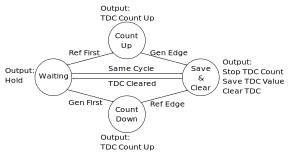
\includegraphics[width=0.8\textwidth]{../state_trans_new}
	\caption[Example State Transition Diagram for a Moore Machine]{Example State Transition Diagram for a Moore Machine.}
	\label{fig:state_trans_reprint}
\end{figure}

The synchroniser circuits are implemented by a pair of ``D'' flip-flips connected in series, clocked on the \ac{FPGA} clock. This synchroniser works by assuming that metastability will only persist for the duration of one \ac{FPGA} clock cycle as depicted in Figure \ref{fig:synchroniser_behav}. In the case where only one clock signal may experience metastability, two synchronisers are required in order to maintain symmetry in the phase comparison.
\begin{figure}[h]
\centering
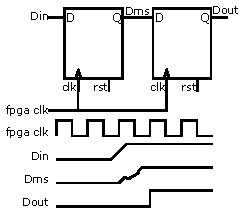
\includegraphics[width=0.4\textwidth]{../synchroniser_behav}
\caption[Double ``D'' flip-flip synchroniser circuit \ac{RTL} diagram]{Double ``D'' flip-flip synchroniser circuit \ac{RTL} diagram.}
\label{fig:synchroniser_behav}
\end{figure}

This \ac{FSM} then controls an Up-Down counter of the same width as the control code, counting in two's complement. As the control code has already been defined as a 7 bit wide two's complement integer, the phase detector's output can theoretically lie in the range $[-64,63]\cap\mathbb{Z}$. 

As this detector samples each signal at the \ac{FPGA} clock frequency, the phase detector resolution is equal to the \ac{FPGA} clock period at:
\begin{equation}
t_{res} = T_{FPGA} = \frac{1}{258\times 10^{6}} = 3.875~\si{\nano\second}
\end{equation}
an angular resolution of:
\begin{equation}
res = \frac{t_{res}}{T_{osc}} \cdot 360\si{\degree} = \frac{3.875~\si{\nano\second}}{200~\si{\nano\second}} \cdot 360\si{\degree} = 6.975\si{\degree}
\end{equation}

The counter is implemented using saturation arithmetic to prevent overflow at high phase differences which could potentially harm the ability of the \ac{ADPLL} to obtain a lock. In the case of this \ac{PD} the phase error at which overflow may occur can be computed using the bit width of the counter and temporal resolution. $error_{max} = 63\cdot3.875~\si{\nano\second} = 244.125~\si{\nano\second}$. As this is greater than the period it cannot occur for purely a phase difference, but may occur in the presence of either a frequency divider in the feedback path, thus increasing the period of the signal used for comparison, or of a significant frequency difference between the signals. When implementing the clamping logic, the decision was taken to make the detection range symmetrical, thus the output range was reduced by one increment to $[-63,63]\cap\mathbb{Z}$.

Figure \ref{fig:updown_ctr} depicts the implementation of this counter. Apart from the aforementioned capping of the measurement range implemented using a pair of comparators and a multiplexer, important to note is the bit width of the increment. Despite overflow being disallowed when the number is interpreted as a signed number, the addition of a 7 bit wide -1 to the accumulator value will cause overflow in the adder. This, however, is perfectly valid as an implementation of subtraction in two's complement. On the right side of the diagram the output register can be seen. Clocked using the \ac{FSM}s measurement interval complete signal, this register preserves the phase error until the termination of the following interval.
\begin{figure}[h]
	\centering
	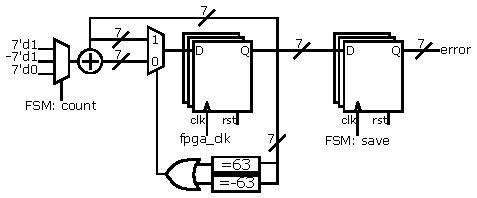
\includegraphics[width=0.8\textwidth]{../updown}
	\caption[\ac{RTL} diagram of up-down counter]{\ac{RTL} diagram of up-down counter.}
	\label{fig:updown_ctr}
\end{figure}

A major pitfall was encountered in this design of phase detector, which lead in some conditions to a form of mode-locking, in which each oscillator would lock $180\si{\degree}$ phase shifted from the oscillators used as a reference. This was later discovered to be as a result of the measurement interval termination conditions in the \ac{FSM}, which in addition to those described in Figure \ref{fig:state_trans_reprint}, would terminate the interval if a falling edge was observed on the signal that originally triggered the measurement. Figure \ref{fig:uncertainty} will be used to describe the exact circumstances of the error.
\begin{figure}[h]
	\centering
	
\includegraphics[width=0.6\textwidth]{../uncertain}
	\caption[Circumstances of mode locking behaviour]{Circumstances of mode locking behaviour.}
	\label{fig:uncertainty}
\end{figure}

The situation would occur when the measurement interval began with a large phase difference between the generated and reference signals and a simultaneous difference in frequency. Without a frequency difference the measurement beginning at ``interval start'' would terminate at location ``a'', measuring a large lag, with the following measurement interval starting at location ``d''. However in the presence of a frequency differential, the rising edge on the generated signal may occur only at location ``c'', and with the falling edge termination condition causing the interval to terminate before this edge was detected, at point ``b''. This lead to a slightly lower magnitude phase lag detected, however this is a minor flaw, and not the cause of the mode locking. As the rising edge at point ``c'' occurs after the interval has terminated, it is treated as a fresh measurement interval, terminating at ``d''. As in this interval, the generated signal has seen the first rising edge, a large lead will be recorded. As each correction is made with a delay of one cycle, in order to avoid timing violations in the feedback path, there is potential for oscillation between lead and lag detection to occur depending on the initial conditions. This low probability behaviour was observed by chance, due to coding error, while using a frequency divider in the feedback path as this ensured the lead and lag measurements were of identical magnitude. 

\subsubsection{Simulations}
%TODO simulations
As this was the first \ac{ADPLL} design implemented, various Vivado test benches were used to verify the behaviour of each module. Simulations with this design were made more efficient due to deterministic timing in all modules, and absence of any inverter based components which required the use of post-implementation simulations in order to avoid zero delay oscillations. Deterministic timing means \ac{ADPLL} 1 offers an additional, and significant, advantage over other designs as it can be entirely simulated in Vivado with accurate timings. This ability was vital initially, as it revealed the presence of edge situations that had not been accounted for, and through exporting the waveforms to a log file and analysis performed using Matlab comparison made to the measured system behaviour.

\begin{figure}[h]
	\centering
	\subfloat[Vivado simulation.]{{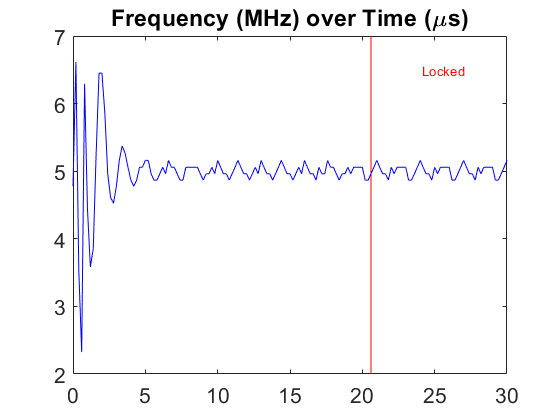
\includegraphics[width=0.45\textwidth]{../sim_locking} }}%
	\subfloat[Hardware measurement.]{{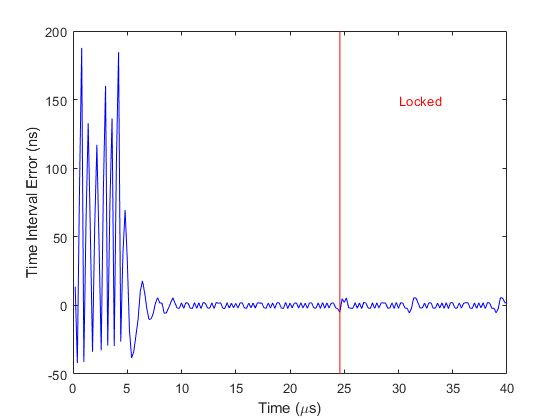
\includegraphics[width=0.45\textwidth]{../impl_locking} }}%
	\caption[\ac{ADPLL} 1 Vivado locking simulations]{\ac{ADPLL} 1 Vivado locking simulations.}
	\label{fig:sim_locking}
\end{figure}
In Figure \ref{fig:sim_locking} (a), the startup behaviour of the system can be observed. This simulation was performed with a reference at exactly $5~\si{\mega\hertz}$ and an initial deviation of $252~\si{\kilo\hertz}$, and the plot shows the inverse of the \ac{DCO} period against the time since the oscillator was enabled. After some initial oscillation the period settles around that of the reference. Once locked, cycle-to-cycle jitter was calculated to be $3.491~\si{\nano\second}$ using the standard deviation of the periods, with a worst case cycle-to-cycle change of $9.299~\si{\nano\second}$. Lock was visually determined to have occurred after $20.91~\si{\micro\second}$, after which the oscillator frequency began to change in a repetitive pattern. later the same test carried in hardware with identical initial conditions, the results of which are shown in Figure \ref{fig:sim_locking} (b). This plot is derived from data captured using an Agilent MSO7054A, using a setup that will be further explained in Section \ref{section:measurement_setup}. Despite lacking a non ideal reference, less violent initial oscillation, and a lesser until lock could be visually determined, the simulation provided a good insight into the system's behaviour once implemented on an \ac{FPGA}.



\subsubsection{\acs{ADPLL} 1 Design Summary}
The listed components were brought together in \textsc{NetworkADPLL.v}, attached in Appendix \ref{adx:code} Listing \ref{lst:network_adpll}. Important to note is that each \ac{ADPLL} only contains two \acl{PD}s despite during network operation the need for phase comparisons to be made with up to four neighbours. The two ``missing'' \ac{PD}s are in fact synthesised as part of the other \ac{ADPLL}s, with which the comparison would be made. This allows for a 50\% reduction in the number of \ac{PD}s required, while also ensuring identical error is received by both \ac{ADPLL}s. Each \ac{ADPLL} performs comparison with the \ac{DCO} ``above'' and ``left'' of them in the Cartesian grid, and a port in the module outputs the results for use by the other \ac{ADPLL}s involved. %TODO juvenile wording
Table \ref{table:adpll1} contains a brief overview of the bit widths, tuning ranges and other configuration information for this \ac{ADPLL}.
\begin{table}[!h]
	\begin{center}
		\begin{tabular}{|l|r|r|r|}
			\multicolumn{4}{c}{\ac{DCO} Tuning Range} \T\\
			\hline
			\multicolumn{1}{|c|}{-} & \multicolumn{1}{c|}{Minimum} & \multicolumn{1}{c|}{Step} & \multicolumn{1}{c|}{Maximum} \T\\
			\hline
			Frequency & $1.008~\si{\mega\hertz}$ & \multicolumn{1}{r|}{$62.988~\si{\kilo\hertz}$} & $8.944~\si{\mega\hertz}$ \T\\
			\hline
			Period & $992.0~\si{\nano\second}$ & \multicolumn{1}{r|}{$2.5~\si{\nano\second}$ (at $5~\si{\mega\hertz}$)} & $111.8~\si{\nano\second}$ \T\\
			\hline
		\end{tabular}
		\begin{tabular}{|l|r|l|r|}
			\multicolumn{4}{c}{Configuration as Implemented} \T\\
			\hline
			\ac{DCO} Counter Width & 12 bits & \ac{DCO} Control Width (max) & 12 bits \T\\
			\hline
			\ac{DCO} Bias Point & 79 & Runtime Gains & Enabled \T\\
			\hline
			Phase Detector Error Width & 7 & Error Sum Weight Width & 4 \T\\
			\hline
			\acs{kp} width & $2^{-5}\times[0,15]\cap\mathbb{Z}$ & \acs{ki} & $2^{-8}\times[0,15]\cap\mathbb{Z}$ \T\\
			\acs{kp} & $2^{-5}\times[0,15]\cap\mathbb{Z}$ & \acs{ki} & $2^{-8}\times[0,15]\cap\mathbb{Z}$ \T\\
			\hline
			Detection Resolution & $3.875~\si{\nano\second}$ & Detection Phase Resolution & $6.975\si{\degree}$ (at $5~\si{\mega\hertz}$)\\
			\hline
		\end{tabular}
	\end{center}
\caption[ADPLL Design 1 Summary]{ADPLL Design 1 Summary.}
\label{table:adpll1}
\end{table}

\subsection{\acs{ADPLL} Design 2}
The second \ac{ADPLL} design implemented during the course of this project was somewhat of a stepping stone between fully synchronous and asynchronous to the \ac{FPGA} clock. The clocked phase detector is reused from above, albeit with an altered error width, while the \ac{DCO} is replaced by a \acl{RO}. While the phase detector was known to work due to testing in \ac{ADPLL} 1, the \ac{DCO} could not be simulated using accurate timings so all testing had to be done in hardware. This presented a challenge, as depending on the implementation, the characteristics of the \ac{DCO} could change, most importantly the centre frequency. The module implementing this \ac{ADPLL} can be found in \textsc{NetworkRingADPLL.v}, attached in Appendix \ref{adx:code} Listing \ref{lst:network_ring_adpll}.

\subsubsection{\acl{DCO}}
\ac{ADPLL} 2 exchanges the \ac{FPGA} clocked oscillator for \ac{RO}, with the aim of obtaining performance more akin to that of an \ac{ASIC} based mixed-signal implementation, due to the variation in period steps both between oscillators and within the same oscillator due to the oscillator layout. Also advantageous is the improvement in period resolution obtained using this design, when compared to that of the \ac{FPGA} clocked design. Taking the formula given in Chapter \ref{chap:3} and the inverter propagation time used by Vivado in post synthesis/implementation simulations of $315~\si{\pico\second}$, the period step can be computed:
\begin{align}
t_{step} &= \text{inverters per step}\times\text{inversions per period}\times\text{propagation delay} \\
t_{step} &= \text{inverters per step}\times\text{inversions per period}\times\tau_{inv} \\
t_{step} &= 2\times 2\times 315~\si{\pico\second} = 1.26~\si{\nano\second}
\end{align}
Using the propagation delay, $\tau_{inv}$, the number of inverters required to produce the signal of period $200~\si{\nano\second}$ can easily be computed:
\begin{equation}
\text{num\_inverters} = \left \lfloor{ T_{osc~@~5~\si{\mega\hertz}}\times \frac{1}{2\times\tau_{inv}}}\right \rceil = \left \lfloor{ \frac{200~\si{\nano\second}}{0.63~\si{\nano\second}}}\right \rceil = 317
\end{equation}

\begin{figure}[h]
	\centering
	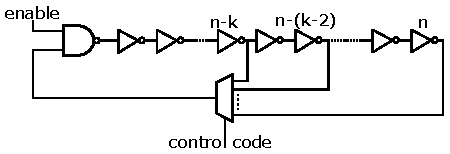
\includegraphics[width=0.8\textwidth]{../ro_new}
	\caption[\acl{RO} RTL diagram]{\acl{RO} RTL diagram.}
	\label{fig:ro_impl}
\end{figure}
Figure \ref{fig:ro_impl} contains an \ac{RTL} diagram of the \ac{RO} as implemented. The inverter chain is specified with a maximum length of $n$ and a maximum number of removable inverters of $k$. In order to preserve the unstable circuit, by maintaining an odd number of inverters, only multiples of two inverters may be removed at a time. The already introduced \ac{DCO} and \ac{PFD} designs all followed the same convention regarding phase error and the corresponding impact on the control code: In the \ac{PFD}, if the generated signal was lagging the reference, meaning it should ``go faster'' in order to ``catch up'', the error given a positive sign. Similarly in the \ac{FPGA} clocked \ac{DCO}, a positive change in the magnitude of the control code resulted in a higher frequency. In the interests of consistency and extensibility the same behaviour was implemented for this \ac{DCO} also, with the number of inverters in the chain given as:
\begin{equation}
\text{num inverters} = n - 2\times CC,~CC<\frac{k}{2}
\end{equation}
Where $CC$ is the unsigned integer control code input. $k$ is determined by the bit width of the control code which, as in the case of the clocked \ac{DCO}, is also an unsigned number. An inverter chain will oscillate freely and cannot be disabled. To this end the first inverter in the chain was replaced by a \acs{NAND} gate to grant control over its operation.

The bias point functions differently in this oscillator, as unlike the \ac{FPGA} clocked design it is not required to set the centre of the tuning range, as in the \ac{RO} this lies at $n-\frac{k}{2}$. Instead the bias point servers as a conversion between the signed \ac{LF} output, which is in two's complement form, and the unsigned requirement of the control code. This is achieved by adding on the midpoint of the unsigned range and storing the result in an unsigned value. Using the case where the width of the control code is three: The range of the signed three bit integer is from $-4$ (100) to $3$ (011) which when directly converted to unsigned values become $4$ and $3$, thus destroying the relationship between lead and lag. Worse still the signed value of $-1$ (111) becomes $7$. Adding on the mid range value solves this problem, with a signed value of $-4$ now mapping to $0$ and $3$ to $7$. Comparing this behaviour to response of the \ac{RO} to the control code, it can be trivially seen that the minimum possible period will still correspond to the largest control code prior to conversion and vice versa for the maximum period.

A control code width of 5 bits was chosen, as with two inverters removed per control code, the tunable range would consist of $20\%$ of the total inverter count. To achieve this range with a centre of $317$ inverters, the maximum number of inverters in the chain was required to be $317+2\times 2^{5-1} = 349$, dropped to a minimum at $285$. The corresponding minimum and maximum frequencies then are:
\begin{align}
f_{osc} &= \frac{1}{T_{osc}} = \frac{1}{(n-2CC)\times 2\times\tau_{inv}} = \frac{1}{(n-2CC)\times 2\times 315~\si{\pico\second}} \\
f_{min} &= \frac{1}{T_{max}} = \frac{1}{349\times 2\times 315~\si{\pico\second}} = 4.548~\si{\mega\hertz} \\
f_{max} &= \frac{1}{T_{min}} = \frac{1}{285\times 2\times 315~\si{\pico\second}} = 5.569~\si{\mega\hertz}
\end{align}

The first pitfall with this type of \ac{DCO} comes in the \ac{HDL} stage, with the \ac{EDA} likely to optimise away what it sees as a long chain of inverters carrying out no function. This can be avoided by adding an \texttt{attribute} as a prefix to the instantiation of a logic element or net that should not be ``optimised'' away. It is important to choose the correct directive, otherwise the compiler may not behave as expected. In the case of Vivado, it is important not to confuse the \texttt{KEEP} or \texttt{KEEP\_HIERARCHY} commands with that of \texttt{DONT\_TOUCH}, with former commands only ensuring that the logic elements will be maintained in synthesis, but not in any subsequent stages \cite{synth_ug}.

As mentioned in previous chapters, the absence of direct control over layout can lead to significant variation of the propagation time though inverters. This may occur in three ways: Firstly, the layout of individual \ac{RO}s may be significantly different, thus resulting in poor overlap of tuning regions. Anecdotally, while implementing a 3x3 network, 7 of the 9 oscillators had centre frequencies within a $100~\si{\kilo\hertz}$ span but two lay more than $500~\si{\kilo\hertz}$ away in opposite directions which prevented the network from locking. Secondly, within an \ac{RO} the propagation delay between each inverter may vary, which results in a variable frequency step, possibly changing the locking range. These two effects represent an extreme version of the variation due to process or manufacturing seen on \ac{ASIC}s. The final variation is possibly the most frustrating, and occurs when between implementations the \ac{EDA}, Vivado in the case of this project, changes the layout of the \ac{RO}. This may occur as a result of a direct change, or as a result of seemingly innocuous changes to unrelated modules. While the final problem can be avoided, once the performance of the \ac{RO} is satisfactory, by locking down module, the remaining two problems can only be mitigated somewhat.

This is achieved by assigning specific areas of the chip in which that module must lie, although these must be of a size approximately $40\%$ larger than the minimum space required in order to avoid having the router create a complex, delay intensive layout to fit the \ac{RO}. To achieve greater consistency, the implementation directive can be modified such that the router will attempt to use the minimum area that does not require complex routing. \texttt{congestion\_spreadlogic\_low} was used for this purpose in this project, although other options may obtain similar results. The other options available in Vivado can be viewed in the \textit{Vivado Design Suite User Guide - Implementation} \cite{impl_ug}.

With the hardware description of the \ac{RO} completed, testing of an instance of the \ac{RO} with a constant control code of zero was attempted, and it was discovered that the estimation of the centre frequency based on the propagation delay was off by $100$s of $\si{\kilo\hertz}$. The addition of 100 inverters was required to restore a centre of $5~\si{\mega\hertz}$. After the \ac{RO} was integrated into \ac{ADPLL} 2 the centre frequency was discovered to have changed once more. The minor variation caused by the now variable control code had changed the average propagation delay through the inverters once more, now requiring 373 inverters for $5~\si{\mega\hertz}$.
%TODO possibily problematic in the last two paragraphs

When, later in the project, additional \ac{RO}s were implemented to form networks, 373 inverters proved a suitable starting point which consistently delivered \ac{DCO}s with a centre frequency within $200~\si{\kilo\hertz}$ of $5~\si{\mega\hertz}$. For the purposes of describing a typical tuning range, the average propagation delay of an \ac{RO} consisting of 373 inverters with a centre frequency of $5.06~\si{\mega\hertz}$ will be used. To avoid the aforementioned issues with constant control codes, the fixed code was achieved by implementing an \ac{ADPLL} and setting the \ac{PI} filter gains to zero at runtime before performing a reset.

Using this updated maximum number of inverters the frequency range can be recalculated. Firstly, the new minimum and maximum numbers of inverters are $309$ and $373$ respectively, with a mid point at $341$. The inverter delay and period step are then recomputed based on the centre frequency of $5~\si{\mega\hertz}$ as:
\begin{align}%TODO 2 x 2 x midpoint justification - in prev. chapter?
t_{step} &= \frac{T_{osc}}{0.5\times(n-\frac{k}{2})} = \frac{200\si{\nano\second}}{0.5\times 341} = 1.176~\si{\nano\second} \\
\tau_{inv} &= \frac{t_{step}}{2\times\text{inverters per step}} = \frac{t_{step}}{2\times2} = \frac{1.176~\si{\nano\second}}{4} = 293~\si{\pico\second}
\end{align}
The frequency range is then:
\begin{align} 
f_{osc} &= \frac{1}{T_{osc}} = \frac{1}{(n-2CC)\times 2\times\tau_{inv}} \\
f_{min} &= \frac{1}{T_{max}} = \frac{1}{(373-0)\times 2\times 293~\si{\pico\second}} = 4.571~\si{\mega\hertz} \\
f_{max} &= \frac{1}{T_{min}} = \frac{1}{(373-2\times32)\times 2\times 293~\si{\pico\second}} = 5.518~\si{\mega\hertz}
\end{align}

The module implementing the \ac{RO} can be found in \textsc{RingOsc.v}, attached in Appendix \ref{adx:code} Listing \ref{lst:ring_osc}.

\subsubsection{Phase Detector}
The \ac{PFD} used in this oscillator is, apart from the bit width of the counter, identical to that used in the previous design. The reduction in counter width will have no impact of performance of the \ac{ADPLL} once a lock has been acquired, however, the capture speed will be reduced for large phase differences due to the counter reaching saturation point significantly sooner. 5 bits corresponds to a counter range of $[-15,15]\cap\mathbb{Z}$, which will saturate at a time delay of $15\times3.875\si{\nano\second} = 58.125~\si{\nano\second}$, a phase lead or lag of $\frac{}{}\times360\si{\degree} = 104.4\si{\degree}$ at $5~\si{\mega\hertz}$. This is an adequate range, as saturation will occur well outside of the normal operating range. This reduction is most noticeable when a divider is active in the feedback path, however during locked operation a phase shift of $58.125~\si{\nano\second}$ will not occur, so this impact is only felt during acquisition.

\subsubsection{\acs{ADPLL} 2 Design Summary}
As previously mentioned, \ac{ADPLL} 2 represents a midway point between \ac{FPGA} clocked designs and those which are asynchronous. As the source of the asynchronicity is the inverter chain \ac{DCO}, a more realistic jitter would be expected from this design, with there being a significant distribution of period steps. Among other aspects, this will have a noticeable impact in steady state conditions, where the degree of fractional synthesis required will vary from oscillator to oscillator depending on the closest distance from the reference period to a period obtainable by the individual oscillator. This is a source of jitter that was not present in the clocked \ac{DCO} used in \ac{ADPLL} 1, as all period steps were equal. Once again the \ac{DCO} tuning ranges and configuration details for future measurements are listed below, in Table \ref{table:adpll2}.

\begin{table}[!h]
	\begin{center}
		\begin{tabular}{|l|r|r|r|}
			\multicolumn{4}{c}{\ac{DCO} Tuning Range} \T\\
			\hline
			\multicolumn{1}{|c|}{-} & \multicolumn{1}{c|}{Minimum} & \multicolumn{1}{c|}{Step} & \multicolumn{1}{c|}{Maximum} \T\\
			\hline
			Frequency & $4.571~\si{\mega\hertz}$ & $29.180~\si{\kilo\hertz}$ (at $5~\si{\mega\hertz}$) & $5.518~\si{\mega\hertz}$ \T\\
			\hline
			Period & $218.2~\si{\nano\second}$ & $1.176~\si{\nano\second}$ & $181.1~\si{\nano\second}$ \T\\
			\hline
		\end{tabular}
		\begin{tabular}{|l|r|l|r|}
			\multicolumn{4}{c}{Configuration as Implemented} \T\\
			\hline
			\ac{RO} num. of inverters (max) & 373 & \ac{RO} Control Width & 5 bits \T\\
			\hline
			\ac{RO} Bias Point & 16 & Runtime Gains & Enabled \T\\
			\hline
			Phase Detector Error Width & 5 & Error Sum Weight Width & 4 \T\\
			\hline
			\acs{kp} width & $4$ & \acs{ki} & $6$ \T\\
			\hline
			\acs{kp} & $2^{-4}\times[0,15]\cap\mathbb{Z}$ & \acs{ki} & $2^{-6}\times[0,15]\cap\mathbb{Z}$ \T\\
			\hline
			Detection Resolution & $3.875~\si{\nano\second}$ & Detection Phase Resolution & $6.975\si{\degree}$ (at $5~\si{\mega\hertz}$)\\
			\hline
		\end{tabular}
	\end{center}
	\caption[\ac{ADPLL} Design 2 Summary]{\ac{ADPLL} Design 2 Summary.}
	\label{table:adpll2}
\end{table}


\subsection{\acs{ADPLL} Design 3}
\acs{ADPLL} Design 3 has no dependence on the clock provided by the \ac{FPGA}'s clock management utility, as both the \ac{RO} and the \ac{TDC} are designed using inverters, while a Bang-Bang detector replaces the \ac{FPGA} clock reliant \ac{FSM} of the two previous designs. This introduces a second source of implementation based variation between \ac{ADPLL}s, however, this has significantly lesser impact on the frequency range of the oscillator and no impact on the centre frequencies. The lack of an \ac{FPGA} clocked element results means this design will have the closest behaviour to that of an \ac{ASIC} based \ac{ADPLL} implementation, although as the level of variation due to implementation is much larger on an \ac{FPGA}, the impact of non-idealities will be exaggerated.
%same interface
In order to allow quick exchange of \ac{PD}s or other modules, the module in which this \ac{ADPLL} is implemented is still retains the \ac{FPGA} clock as an input. In fact, this module shares its implementation with that of \ac{ADPLL} 2, as while the \ac{PD} designs are drastically different, the interface is identical. The module implementing this \ac{ADPLL} can be found in \textsc{NetworkRingADPLL.v}, attached in Appendix \ref{adx:code} Listing \ref{lst:network_ring_adpll}.

\subsubsection{\acl{DCO}}
The \ac{DCO} used in \ac{ADPLL} 3 is identical in form to that used in \ac{ADPLL} 2, so the tuning range, period step and all effects of implementation variations carry over to this \ac{ADPLL}. The decision to leave the \ac{RO} unmodified is an easy one, as the intended centre frequency is the same and changing the control code width would remove the ability to fix the cells of each \ac{RO}. Fixing the cells is beneficial as it will maintain the oscillator layout between implementation ``runs'', and thus allow for a better comparison between designs 1 \& 2.

\subsubsection{Phase Detector}
Instead of an \ac{FPGA} clocked phase detector, \ac{ADPLL} 3 uses the modified Bang-Bang detector and \ac{TDL} approach to phase comparison seen in Section \ref{section:signum}. Sign detection is implemented exactly as described in that section, with the double \ac{SR} latch approach used to determine the sign of the phase error. A flip-flop is inserted after the second \ac{SR} latch, clocked on the signal \texttt{done}, which holds the output value and ensures that the sign changes at the same time as the magnitude. The previous discussion of this phase detector proposed no implementation of the edge detectors, which are easily implemented using flip-flops clocked on the signal of interest, with a constant $1$ on the $D$ input. In this form the edge detector is single use only, as subsequent edges will not cause any change in the flip-flop output. This is important as it ensures the measurement interval will only terminate when a rising edge is seen on the signal that did not start the measurement interval, thus avoiding the mode locking seen in the original implementation of the \ac{FPGA} clocked \ac{PD}. Once the measurement interval has completed, the \texttt{done} signal is used to reset the edge detectors asynchronously. It is possible that an edge may occur within the time taken to reset the counters, and thus the detector incorrectly gauge the start of a measurement interval, however this can only occur in exceptional circumstances in the acquisition period. Therefore it is possible to ignore this scenario, as the only impact will be an increased time taken to acquire a lock.
\begin{figure}[h]
	\centering
	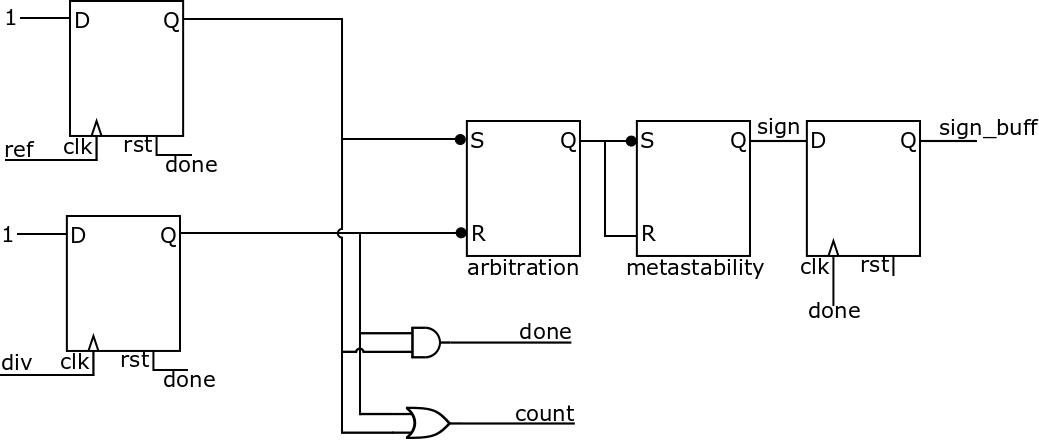
\includegraphics[width=0.8\textwidth]{../new_pdet1}
	\caption[Modified Bang-Bang sign detector RTL diagrams]{Modified Bang-Bang sign detector RTL diagrams.}
	\label{fig:signdet_impl}
\end{figure}

A two signal interface controls the \ac{TDC}, a \texttt{count} that enables the \ac{TDC} and a \texttt{done} signal that signals the termination of the interval. A single logic gate is required to generate each signal, as ORing the two edge detector outputs will produce logic $1$ when the interval has begun while ANDing these signals will indicate the end of the interval when both edges have occurred. The \texttt{done} signal is also used to clock the flip-flop acting as a buffer for the sign. The exact implementation of the sign detection circuit can be seen in Figure \ref{fig:signdet_impl}.

As previously mentioned, the time-to-digital conversion is carried out by a tapped delay line. As with the \ac{RO}, inverters will be used to provide the delay between each tap, and thus the resolution of the \ac{TDL} and the length of each individual delay is based on the layout chosen by the router in Vivado. Due to this, the exact resolution of the phase detector is unknown, although the delay through inverters used in Vivado simulations and the average delay computed based on \ac{RO} centre frequencies can be used to estimate that of the phase detectors. Based these figures for the the propagation delay due to an inverter, $\tau_{inv}$ can be estimated to be in the region of $300~\si{\pico\second}$. As each tap consists of an inverter pair, the delay through the tap, $\tau_{tap} \approx 600~\si{\pico\second}$. Characterisation of the \ac{TDL}, and thus measurement of the delays in each \ac{TDL}, is technically possible, however, this is an time consuming process as many \ac{TDL}s would need to be characterised in order to accurately compute the average delay. 

%TODO eugene
The delay line itself is shown in Figure \ref{fig:tdl_impl}, with each tap implemented by a pair of flip-flops and three inverters. For an $N$ bit width phase error detection, $2^{N-1}-1$ taps are required. In the case of this \ac{ADPLL}, a 5 bit two's complement error signal is required, thus the range of the signal is $[-16,15]\cap\mathbb{Z}$. If the range is made symmetrical, 15 taps are required to fill a signal of this size. From the diagram it can be seen that unless edges are detected on each signal at exactly the same instant, it is almost impossible to measure a zero phase difference between reference and generated signals. This is an intentional decision, \cite{idkwhattocite}.
\begin{figure}[h]
	\centering
	
\includegraphics[width=1.0\textwidth]{../new_pdet2}
	\caption[Inverter based \ac{TDL} RTL diagrams]{Inverter based \ac{TDL} RTL diagrams.}
	\label{fig:tdl_impl}
\end{figure}
The operation of the \ac{TDL} is as follows: A delayed version of the \texttt{count} signal acts as the clock for flip-flops forming each tap, which are rising edge activated. These flip-flops have a constant ``1'' at their $D$ inputs, so as the signal propagates through the delay line, each flip-flop with propagate a logic ``1'' to their corresponding \texttt{error\_tap[i]} signal. When the measurement interval has completed, the \texttt{count} signal clocks the 15 bit wide \texttt{error\_tap} signal into \texttt{error\_tap\_buff} which act as the output buffers of the \ac{PD}, holding the phase error constant between measurement intervals. As with the flip-flops performing edge detection, the flip-flops comprising the taps can only be used once before requiring a reset, which is again carried out using the \texttt{done} signal. As flip-flops have a hold time, the duration after the clock edge in which the signal applied at the $D$ input must not change to ensure valid data, an inverter is used to delay the reset to avoid this issue.

The output of the \ac{TDL} itself is not a binary signal, but rather the thermometer coded representation of the number of taps activated in the measurement interval. In order to convert to binary, the easiest solution is a switch statement, with an assignment performed based on the temperature code. However all \ac{ADPLL} blocks have been designed to be extensible, requiring the lookup to be generated at compile time. This is somewhat difficult to implement, and a simpler solution exists for this problem. In a \texttt{generate} statement, a variable size loop is used to count the number of nonzero bits as it would be done in C. At compile time this loop is converted into lookup tables, similarly to the switch statement.

The now unsigned binary representation of the error magnitude can be combined then with the sign bit to form a two's complement error signal. The file \textsc{PhaseDetectorDL.v} in Appendix \ref{adx:code} Listing \ref{lst:phase_detector_dl} contains the Verilog implementation of this module. \texttt{DONT\_TOUCH} compiler directives were used here in a number of places to ensure that the inverters and other elements that are key for timing are not removed in the synthesis process, as similarly to \ac{RO}, Vivado sees these as unneeded elements serving no purpose.

\subsubsection{\acs{ADPLL} 3 Design Summary}
Compared to the oscillators suggested earlier, \ac{ADPLL} 3 achieves a significantly finer detection resolution, at the expense of significant variation in the detection step. This can be viewed as advantageous however, as the \ac{ADPLL} exhibits an exaggerated version of the implementation and manufacturing defect based variability present in an \ac{ASIC}. It is this type of \ac{ADPLL} that both the \acs{UCD} and Sorbonne research teams are using to examine potential designs and test theoretical results. As before, Table \ref{table:adpll3} presents the important numeric characteristics of this \ac{ADPLL}.


\begin{table}[!h]
	\begin{center}
		\begin{tabular}{|l|r|r|r|}
			\multicolumn{4}{c}{\ac{DCO} Tuning Range} \T\\
			\hline
			\multicolumn{1}{|c|}{-} & \multicolumn{1}{c|}{Minimum} & \multicolumn{1}{c|}{Step} & \multicolumn{1}{c|}{Maximum} \T\\
			\hline
			Frequency & $4.571~\si{\mega\hertz}$ & $29.180~\si{\kilo\hertz}$ (at $5~\si{\mega\hertz}$) & $5.518~\si{\mega\hertz}$ \T\\
			\hline
			Period & $218.2~\si{\nano\second}$ & $1.176~\si{\nano\second}$ & $181.1~\si{\nano\second}$ \T\\
			\hline
		\end{tabular}
		\begin{tabular}{|l|r|l|r|}
			\multicolumn{4}{c}{Configuration as Implemented} \T\\
			\hline
			\ac{RO} num. of inverters (max) & 373 & \ac{RO} Control Width & 5 bits \T\\
			\hline
			\ac{RO} Bias Point & 16 & Runtime Gains & Enabled \T\\
			\hline
			Phase Detector Error Width & 5 & Error Sum Weight Width & 4 \T\\
			\hline
			\acs{kp} width & $4$ & \acs{ki} & $6$ \T\\
			\hline
			\acs{kp} & $2^{-4}\times[0,15]\cap\mathbb{Z}$ & \acs{ki} & $2^{-6}\times[0,15]\cap\mathbb{Z}$ \T\\
			\hline
			Detection Resolution & $\approx0.63~\si{\nano\second}$ & Detection Phase Resolution & $1.134\si{\degree}$ (at $5~\si{\mega\hertz}$)\\
			\hline
		\end{tabular}
	\end{center}
	\caption[\ac{ADPLL} Design 3 Summary]{\ac{ADPLL} Design 3 Summary.}
	\label{table:adpll3}
\end{table}

\section{Measurement Setup}\label{section:measurement_setup}
For the following sections in which the performance of either individual \ac{ADPLL}s or \ac{ADPLL} networks the same measurement setup was used. The \ac{FPGA} used was a Xilinx Artix-7 \acl{Nexys} on a Digilent \acs{Nexys} board. The \acl{Nexys} features 15850 logic slices, each with 4 lookup tables and 8 flip-flops. There are six clock management tiles, 240 dedicated digital signal processing slices and an analog-to-digital converter. The maximum operating frequency is $464~\si{\mega\hertz}$ and 210 input/output ports are available for use. Further information can be found in the datasheet \cite{a7_datasheet}. The \acs{Nexys} is an evaluation/development board for the aforementioned \ac{FPGA}, however directed at the education sector. It contains useful peripherals such as 16 switches, 8 7-segment displays and 4 user addressable \ac{PMOD} headers and can be used with the free of charge ``Webpack'' version of Vivado \cite{n4_datasheet}.
\begin{figure}[h]
	\centering
	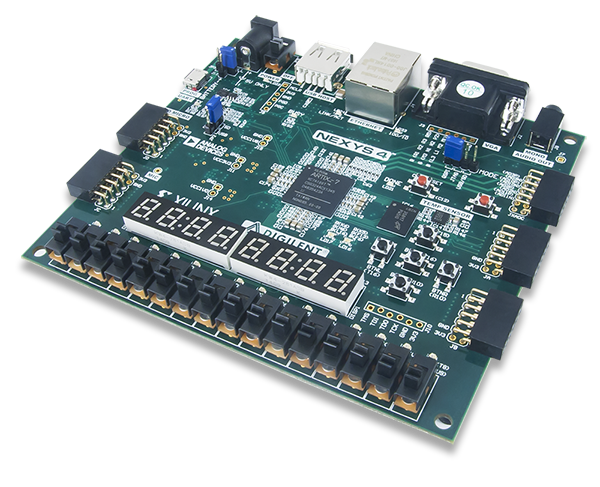
\includegraphics[width=0.6\textwidth]{../n4}
	\caption[\acs{Nexys} development board]{\acs{Nexys} development board.}
	\label{fig:n4}
\end{figure}

Measurements were performed using an Agilent MSO7054A, a four channel, $4~\si[per-mode=symbol]{\giga\sample\per\second}$ oscilloscope. Signals were extracted over the regular \ac{PMOD} headers as the board does not provide outputs better suited to the measurement of signals that are available to the user, such as SMA or BNC connectors, and the \ac{PMOD} header for the analog-to-digital converter, which has lower impedance traces, is not available for the designer to re-configure. Data was acquired with the oscilloscope in quad channel mode at a sampling rate of $2\si[per-mode=symbol]{\giga\sample\per\second}$. One of the four channels was consumed by the external reference, leaving three free for signal measurements, in most cases the generated output of three \ac{ADPLL}s were connected. $200\si{\micro\second}$ long captures were saved to an Agilent specified binary format which could be opened in Matlab for analysis.
%TODO diagram or picture of some sort

\section{\acs{ADPLL} Characterisation}
%TODO why each PLL

% //9 for older tests @1111 = 4@0000, but >> 5 cos of extra size
% <4 is a no can do //7 for older tests @1111 = 4@0001

\section{Minor Variations}\label{section:minor_variations}
%TODO osc size

\section{\acs{ADPLL} Network Implementation}
\subsection{2x2 Network}
\subsection{3x3 Network}
